\documentclass[aspectratio=169,10pt]{beamer}
\usetheme{Madrid}

\usepackage{fancybox,graphicx,hyperref,url}
\usepackage{tikz}
\usetikzlibrary{shapes,arrows}
\usetikzlibrary{positioning}
%\usepackage[T1]{fontenc}
\usepackage{booktabs}
\usepackage{enumitem}
\setbeamercovered{transparent}

\setlistdepth{9}
\setlist[itemize,1]{label=$\bullet$}
\setlist[itemize,2]{label=$\bullet$}
\setlist[itemize,3]{label=$\bullet$}
\setlist[itemize,4]{label=$\bullet$}
\setlist[itemize,5]{label=$\bullet$}
\setlist[itemize,6]{label=$\bullet$}
\setlist[itemize,7]{label=$\bullet$}
\setlist[itemize,8]{label=$\bullet$}
\setlist[itemize,9]{label=$\bullet$}
\renewlist{itemize}{itemize}{9}

\setlist[enumerate,1]{label=$\arabic*.$}
\setlist[enumerate,2]{label=$\alph*.$}
\setlist[enumerate,3]{label=$\roman*.$}
\setlist[enumerate,4]{label=$\arabic*.$}
\setlist[enumerate,5]{label=$\alpha*$}
\setlist[enumerate,6]{label=$\roman*.$}
\setlist[enumerate,7]{label=$\arabic*.$}
\setlist[enumerate,8]{label=$\alph*.$}
\setlist[enumerate,9]{label=$\roman*.$}
\renewlist{enumerate}{enumerate}{9}

\AtBeginSection[]{
  \begin{frame}[noframenumbering]
  \vfill
  \centering
  \begin{beamercolorbox}[sep=8pt,center,shadow=true,rounded=true]{title}
    \usebeamerfont{title}\insertsectionhead\par%
  \end{beamercolorbox}
  \vfill
  \end{frame}
}

\title[Lambda Calculus in a hurry]{Lambda Calculus in a hurry}

\author[Rafael Castro]{
  Rafael Castro G. Silva\\\medskip
  {\small \url{rasi@di.ku.dk}}}

\date{29/06/2022}

\institute[UCPH]{
  Department of Computer Science \\
  University of Copenhagen}

\begin{document}

\begin{frame}
  \titlepage

\end{frame}

\begin{frame}[fragile]
  \frametitle{Motivation}
  \begin{itemize}
    \item Lambda Calculus is very important in Computer Science!
          \pause
    \item Its has many applications in Computer Science
          \begin{itemize}
            \item Do you know any?
          \end{itemize}
          \pause
    \item No prerequisites to learn it (maybe just Set Theory)
          \pause
    \item It sounds really cool
  \end{itemize}
\end{frame}

\begin{frame}{Contents}
  \begin{itemize}
    \item A bit of history
    \item What is and is not a lambda term?
    \item How do we compute?
    \item What cool things can we do with it?
  \end{itemize}
\end{frame}

\begin{frame}{Learning Outcomes}
  \begin{itemize}
    \item Learn some background history about Logic and Computer Science
    \item Identify well-formed terms in Lambda Calculus
    \item Apply beta-reduction to terms
    \item Write down/design your own programs in Lambda Calculus
  \end{itemize}
\end{frame}

\section{A bit of history}

\begin{frame}
  \frametitle{Set Theory}
  \begin{columns}
    \begin{column}{0.75\textwidth}
      \begin{itemize}
        \item A set is a collection of elements
              \begin{itemize}
                \item Unique elements
                \item The order of the elements in the set doesn't matter
                \item Examples:
                      \begin{itemize}
                        \item Numbers
                        \item We in this room
                        \item The set of all sets
                      \end{itemize}
              \end{itemize}
              \pause
        \item A very simple foundation for mathematics
      \end{itemize}
    \end{column}
    \begin{column}{0.2\textwidth}
      \begin{figure}
        \shadowbox{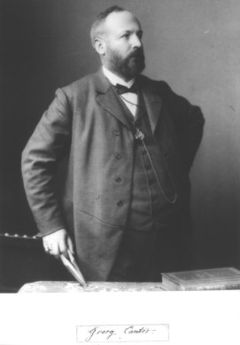
\includegraphics[width=0.35\textwidth]{Georg_Cantor.jpg}}
        \caption{George Cantor}
      \end{figure}
    \end{column}
  \pause
  \end{columns}
  \begin{block}{Russel's Paradox: Set Theory is broken!}
    \begin{columns}
      \begin{column}{0.65\textwidth}
        \begin{align*}
          \text{Let } R = \{x \mid x  \notin x\} \text{, then } R \in R \iff R\not \in R
        \end{align*}
      \end{column}
      \begin{column}{0.25\textwidth}
        \begin{figure}
          \shadowbox{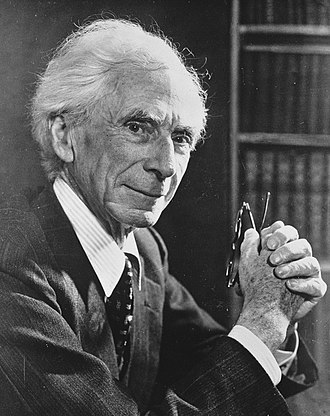
\includegraphics[width=0.30\textwidth]{Bertrand_Russell.jpg}}
          \caption{Bertrand Russel}
        \end{figure}
      \end{column}
    \end{columns}
  \end{block}
\end{frame}

\begin{frame}
  \frametitle{The Problem}
  \begin{block}{The Problem}
    You are David Hilbert and Mathematics is broken
  \end{block}
  \pause

  \begin{columns}
    \begin{column}{0.75\textwidth}
      \begin{block}{Hilbert's Program}
        \begin{itemize}
          \item Provide a new foundation form mathematics
                \begin{itemize}
                  \item The system must be powerful enough to do arithmetic
                  \item Provide a proof that the system is consistent
                  \item \textbf{Provide an algorithm that solves any given problem stated in this system}
                \end{itemize}
                \pause
          \item What do we need here?
                \begin{itemize}
                  \item What is an algorithm?
                \end{itemize}
        \end{itemize}
      \end{block}
    \end{column}
    \begin{column}{0.2\textwidth}
      \begin{figure}
        \shadowbox{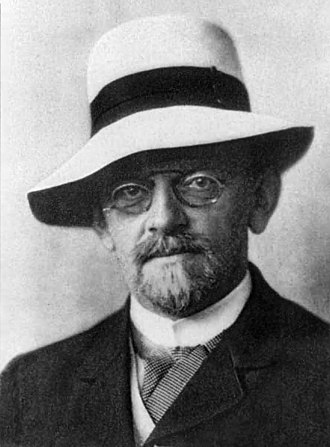
\includegraphics[width=0.35\textwidth]{Hilbert.jpg}}
        \caption{David Hilbert}
      \end{figure}
    \end{column}
    \pause
  \end{columns}
\end{frame}

\begin{frame}
  \frametitle{The Formal Definition of Algorithm}
  \begin{itemize}
    \item Three formal definitions of algorithm showed up together
          \begin{itemize}
            \item \textbf{Alonzo Church: Lambda Calculus in 1935}
                  \begin{itemize}
                    \item It's a language
                  \end{itemize}
                  \begin{figure}
                    \shadowbox{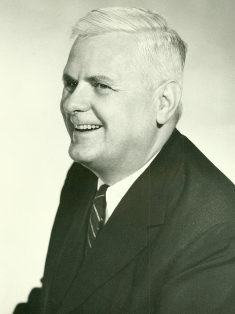
\includegraphics[width=0.05\textwidth]{Alonzo_Church.jpg}}
                  \end{figure}
            \item Kurt Gödel: Recursive Functions in 1935
                  \begin{itemize}
                    \item It's a class of functions
                  \end{itemize}
                  \begin{figure}
                    \shadowbox{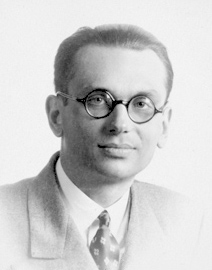
\includegraphics[width=0.05\textwidth]{Kurt_godel.jpg}}
                  \end{figure}
            \item Alan Turing: Turing Machines in 1936
                  \begin{itemize}
                    \item It's an abstract machine
                  \end{itemize}
                  \begin{figure}
                    \shadowbox{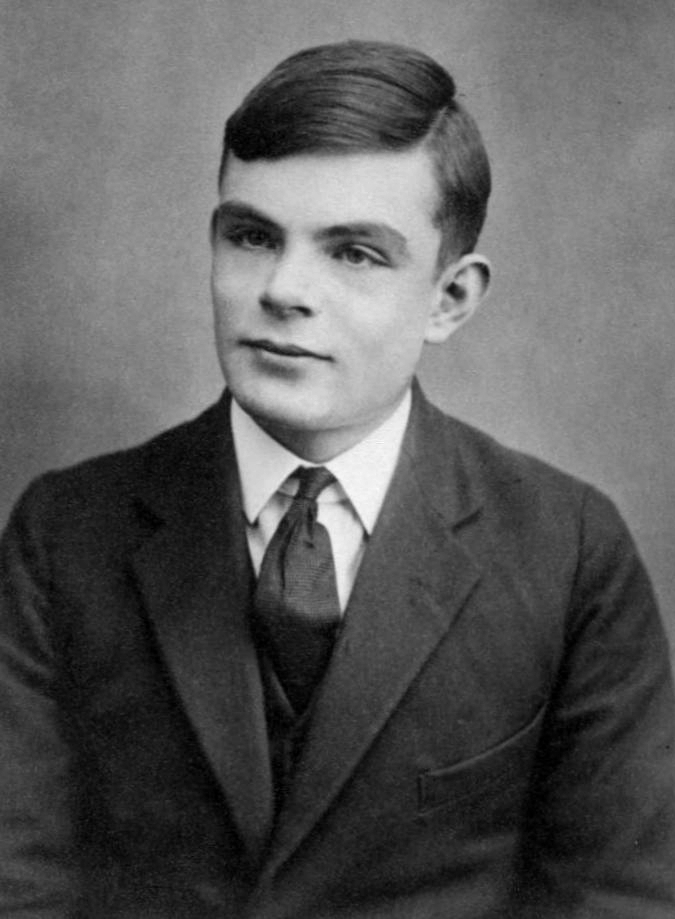
\includegraphics[width=0.05\textwidth]{Alan_Turing.jpg}}
                  \end{figure}
          \end{itemize}
  \end{itemize}
\end{frame}

\section{What is and is not a lambda term?}

\begin{frame}{The Syntax of Lambda Calculus}
  Given a set of variables $V$, a  $\lambda$-term is inductively defined by:

  \begin{itemize}
    \item All variables: $x, y, z, w... \in V$ (atoms) are $\lambda$-terms
    \item If $M$ is a $\lambda$-term and $x$ is a variable, then $\lambda x.M$ is a $\lambda$-term. ($\lambda$ abstraction or $\lambda$ function)
    \item If $M$ and $N$ are $\lambda$-terms, then $(MN)$ is a $\lambda$-term. (application)
  \end{itemize}

  Parenthesis omission convention: $(MN)P \equiv MNP$ for any given $M, N$ and $P$.

  \pause

  \begin{block}{Examples}

    Considering $V \equiv \{x,y,z\}$,
    \begin{enumerate}
      \item $x$
      \item $y$
      \item $z$
      \item $\lambda x.x$
      \item $\lambda x.y$
      \item $(\lambda x.x)y$
      \item $(\lambda x.x)(\lambda x.x)$
    \end{enumerate}
  \end{block}
\end{frame}

\begin{frame}{Exercise 1 (Individual and in 5 min)}
  Which of these are well-formed $\lambda$-terms?

  \begin{columns}
    \begin{column}{0.45\textwidth}
      Considering $V \equiv \{x,y\}$,
      \begin{enumerate}
        \item $x$
        \item $x(\lambda x.x)$
        \item $MNP$
        \item $\lambda x.y$
        \item $\lambda x. \lambda y.xy$
        \item $z$
        \item $(\lambda y.y)(\lambda y.yx)$
      \end{enumerate}
    \end{column}
    \begin{column}{0.45\textwidth}
      \begin{block}{Syntax definition}

        Given a set of variables $V$, a  $\lambda$-term is inductively defined by:

        \begin{itemize}
          \item All variables: $x, y, z, w... \in V$ (atoms) are $\lambda$-terms
          \item If $M$ is a $\lambda$-term and $x$ is a variable, then $\lambda x.M$ is a $\lambda$-term. ($\lambda$ abstraction or $\lambda$ function)
          \item If $M$ and $N$ are $\lambda$-terms, then $(MN)$ is a $\lambda$-term. (application)
        \end{itemize}

        Parenthesis omission convention: $(MN)P \equiv MNP$ for any given $M, N$ and $P$.
      \end{block}
    \end{column}
  \end{columns}
\end{frame}

\section{How do we compute?}

\begin{frame}{Free variables}
  The set of all free variables of $M$, called $FV(M)$, is defined inductively by:
  \begin{align*}
    FV(x) &= \{x\} \\
    FV(MN) &= FV(M) \cup FV(N) \\
    FV(\lambda x.M) &= FV(M) \setminus \{x\}
  \end{align*}

  \begin{block}{Examples}
    \begin{itemize}
      \item $FV(x) = \{ x \}x$
      \item $FV(xy) = \{ x, y\}$
      \item $FV(\lambda x.x) = \emptyset$
      \item $FV(\lambda x.xy) = \{y\}$
    \end{itemize}
  \end{block}
\end{frame}

\begin{frame}{Beta Reduction}
  \begin{block}{Substitution}
    \begin{itemize}
      \item $ [N/x]x \equiv N ; $
      \item $ [N/x]y \equiv y, \: \text{if}\: x \not\equiv y; $
      \item $ [N/x](PQ) \equiv ([N/x]P[N/x]Q) ; $
      \item $ [N/x](\lambda x.P) \equiv \lambda x.P ; $
      \item $ [N/x](\lambda y.P) \equiv \lambda y.P, \: \text{if}\: x \notin FV(P) ; $
      \item $ [N/x](\lambda y. P) \equiv \lambda y.[N/x]P, \: \text{if}\: x \in FV(P) \:\text{and}\: y \notin FV(N) ; $
      \item $ [N/x](\lambda y. P) \equiv \lambda z.[N/x][z/y]P, \: \text{if}\: x \in FV(P) \ :\text{and}\: y \in FV(N) ; $
    \end{itemize}
  \end{block}
  \pause

  \begin{block}{Beta Reduction}
    A term of the form $(\lambda x.M)N$ is called a redex $\beta$ and is interpreted by the substitution $[N/x]M$
  \end{block}
\end{frame}

\begin{frame}{Beta Reduction Examples}
  \begin{block}{Examples}
    \begin{itemize}
      \item $(\lambda x.x)y$
      \item $(\lambda x.x)(\lambda x.x)$
      \item $(\lambda x. \lambda y . y)y$
      \item $(\lambda x. \lambda y . x y)y$
    \end{itemize}
  \end{block}
\end{frame}

\begin{frame}{Beta Reduction Exercise (group and in 5 minutes)}
  \begin{block}{Exercise}
    \begin{itemize}
      \item $((\lambda x.x)(\lambda x.x))(\lambda x.x)$
      \item $(\lambda x.xx)(\lambda x.xx)$
    \end{itemize}
  \end{block}
\end{frame}

\section{What cool things can we do with it?}

\begin{frame}{Let's program}
  \huge{open: www.haskell.org}

\end{frame}

\end{document}
